
\documentclass[12pt]{beamer}
%\documentclass[handout]{beamer}

\usetheme[language=english,framenumber,totalframenumber]{AlleghenyCollege}
\usepackage{biblatex}
\addbibresource{cite.bib}
\title{Shopping Cart}

\author{Isabella Martinez,Travis Thomas, Daniel O'Campo, Jacob Shick}
\date{\today}

   
\begin{document}

\begin{frame}
  \titlepage
   \begin{center}
        
        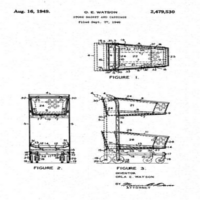
\includegraphics[width=.30\textwidth]{images/test.png}

    \end{center}
  
  
  
\end{frame}

%%%%%%%%%%%% Slide %%%%%%%%%%%%%%%%%%%%%%%%%%%%%%%%%%%%%%%%%%%%%%%%%%%
\begin{frame}
  \frametitle{Market Research}
 	\begin{itemize}
        \item{\large Dennis Curtin, director of public relations at Sunbury, Pa.-based Weis Markets, says that the supermarket chain's average cart costs about \$90[1]} 

    \item {\large An average of 200-250 shopping carts at 100,000 grocery stores}[1]

        \item {\large Average lifespan of shopping cart lasts anywhere from five to seven years}[1]

        \item{\large Wheels can cost anywhere from eight to fourteen dollars each}[2]
        \item { \large One article reads that they should be replaced in two-year cycles}[3]

    \end{itemize}
\end{frame}
%%%%%%%%%%%% Slide %%%%%%%%%%%%%%%%%%%%%%%%%%%%%%%%%%%%%%%%%%%%%%%%%%%
\begin{frame}{Clip image}
\frametitle{Problems with today's shopping carts:  }
\vspace{-1cm}
\textbf{Based on personal opinion and primary sources: }\\
\vspace{.2cm}
\begin{itemize}
      \item {\LARGE Wheels}
        \item { \LARGE Nothing to keep  things cold/Frozen}
        \item {\LARGE No way to organize food}
        \item {\LARGE Requires user interaction} 
    \end{itemize}
\end{frame}
%%%%%%%%%%%% Slide %%%%%%%%%%%%%%%%%%%%%%%%%%%%%%%%%%%%%%%%%%%%%%%%%%%

\begin{frame}


  \frametitle{The Redesign }
 
	\begin{columns}
       \begin{column}{4cm}
       \vspace{-3cm}
            \begin{itemize}
	
     \item The prototype
      \item Features
     \item Frame
    \end{itemize}
         
        \end{column}
    
    
 \begin{column}{7cm}
       \vspace{-1cm}
           \begin{figure}
               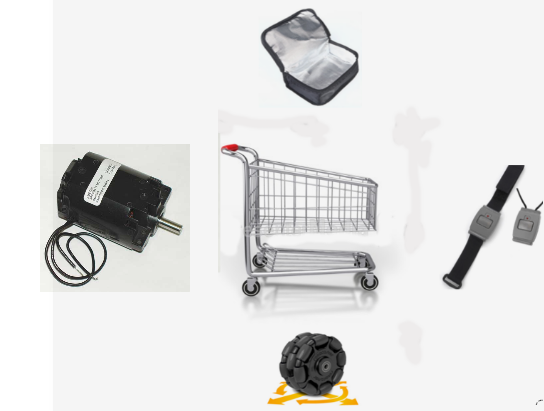
\includegraphics[scale=0.3]{images/design.png}
               
            \end{figure}
        \end{column}
    \end{columns}
\end{frame}
 
%%%%%%%%%%%% Slide %%%%%%%%%%%%%%%%%%%%%%%%%%%%%%%%%%%%%%%%%%%%%%%%%%%











%%%%%%%%%%%%%%%%%%%%%%%%test%%%%%%%%%%%%%%

\begin{frame}
\frametitle{The Redesign }
    \begin{columns}
        \begin{column}{3cm}
            \begin{itemize}
	
      \item Sensor System
      \item Omni-Wheels 
      \item Insulated compartment
    \end{itemize}
          
        \end{column}
        \begin{column}{8cm}
        \vspace{-1cm}
            \begin{figure}
                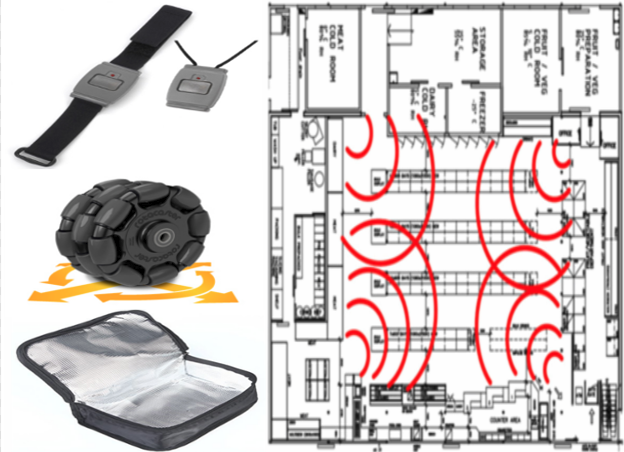
\includegraphics[scale=0.4]{images/Finaldesign.png}
                
            \end{figure}
        \end{column}
    \end{columns}
\end{frame}



%%%%%%%%%%%%%%%%test end %%%%%%%%%%%%%%%%%%%%




\begin{frame}


  \frametitle{Costs per Unit }
 \vspace{-3.0cm}
	\begin{itemize}
	
      \item Basket and Frames: \$40
      \item Wheels: \$60
      \item Insulated Compartment:  \$20
      \item Motor: \$35
      \item Sensor System: One time sensor installation (store dependent) , \$15 per unit
    \end{itemize}
\end{frame}




















%%%%%%%%%%%
%%%%%%%%%%%% Slide %%%%%%%%%%%%%%%%%%%%%%%%%%%%%%%%%%%%%%%%%%%%%%%%%%%
\begin{frame}


  \frametitle{Why would supermarkets buy our cart? }
 \vspace{-2.0cm}
	\begin{itemize}
	
      \item Luxury Item 
      \item Convenience 
      \item Gives “hook ” to a store brand 
      \item Niche Market
    \end{itemize}
    
\begin{figure}
                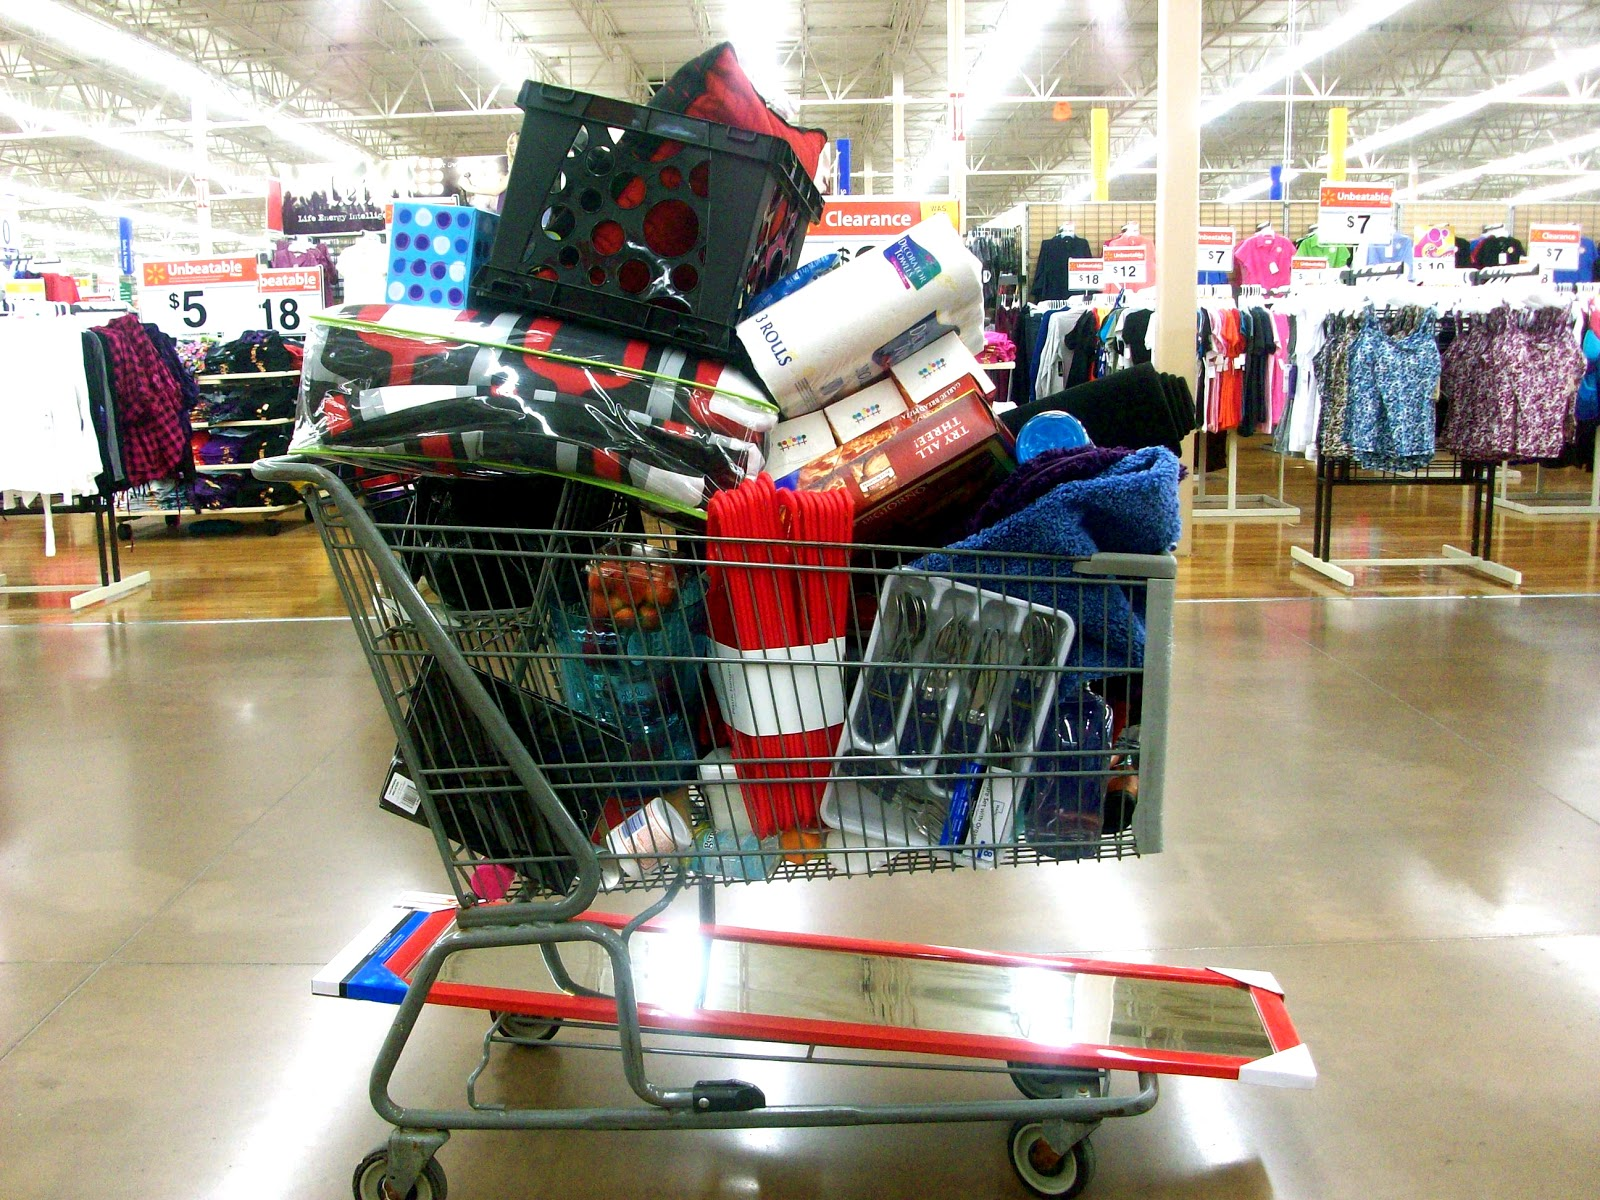
\includegraphics[scale=.05]{images/unorgCart.jpg}
                
            \end{figure}    
    
\end{frame}
%%%%%%%%%%%% Slide %%%%%%%%%%%%%%%%%%%%%%%%%%%%%%%%%%%%%%%%%%%%%%%%%%%







\begin{frame}
 \frametitle{Reference List }
\begin{itemize}
  \vspace{-1.7cm}
 
\item \large\href{http://www.progressivegrocer.com/departments/equipment-design/wheels-fortune
}{\color{blue}{\texttt{{Ingram. (2012). Wheels Of Fortune. Retrieved September 16, 2016}}}}

\item \large \large\href{https://www.uline.com/BL_1887/Standard-Casters}{\color{blue}{\texttt{{Number, B. M. (n.d.). Standard Casters. Retrieved September 16, 2016}}}}


\item \large \large\href{https://caremnt.wordpress.com/2015/05/21/the-lifespan-of-a-shopping-cart-wheel}{\color{blue}{\texttt{{ (2015). The lifespan of a shopping cart wheel. Retrieved September 16, 2016}}}}

\end{itemize}
\end{frame}
%%%%%%%%%%%% Slide %%%%%%%%%%%%%%%%%%%%%%%%%%%%%%%%%%%%%%%%%%%%%%%%%%%











%%%%%%%%%%%% Slide %%%%%%%%%%%%%%%%%%%%%%%%%%%%%%%%%%%%%%%%%%%%%%%%%%%
\begin{frame}
\begin{center}
\Huge
 Thank You!

Questions?

\vspace{0.2in}

\normalsize



\end{center}
\end{frame}


\end{document}
